\subsection{Formato}

Los datos proporcionados por las plataformas tienen un gran volumen, ya que como comentabamos anteriormente, se recolectan
el mayor numero de datos posibles.Este documento contara con multiples muestras para las que
se especifica un conjunto campos. Estos conjuntos de campos son similares entre ellos, pero no tienen por que ser identicos. 
De estos datos, se debera realizar una seleccion de las muestras relevantes, y de estas, los campos necesarios
para su diseno y cuales no.
\newpage

A continuacion podemos ver varios ejemplos tomados del portal de datos abiertos europeo
\footnote{\url{https://tinyurl.com/y3d76525}} 
y norte americano\footnote{\url{https://data.cityofnewyork.us/api/views/kku6-nxdu/rows.json?accessType=DOWNLOAD}}.

\begin{figure}[h]
    \centering
    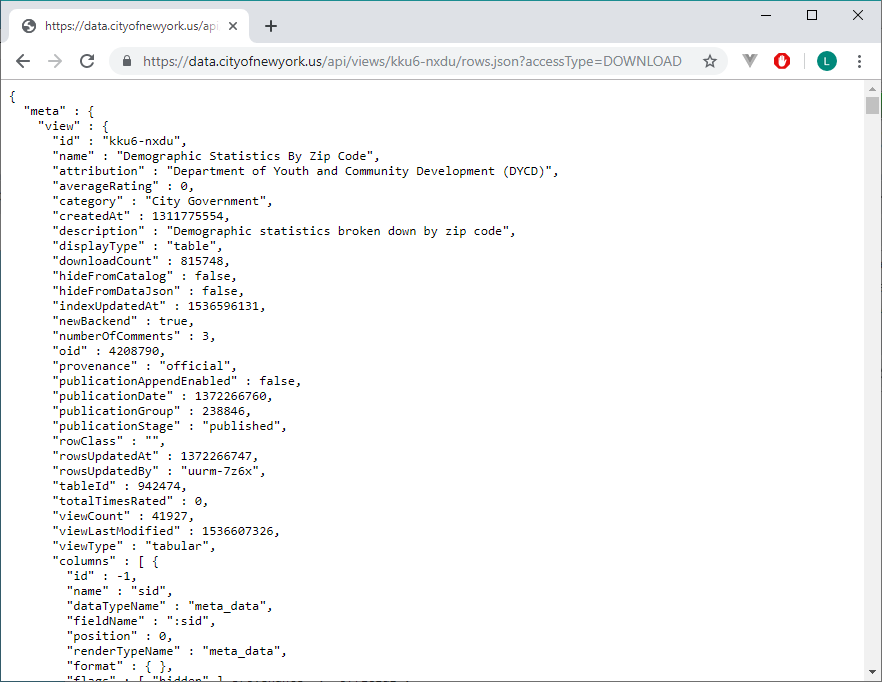
\includegraphics[width=8cm]{ExampleOpenDataEEUU}
    \caption{EEUU Open Portal.Demographic Statistics By Zip Code}
    \end{figure}

    \begin{figure}[h]
    \centering
    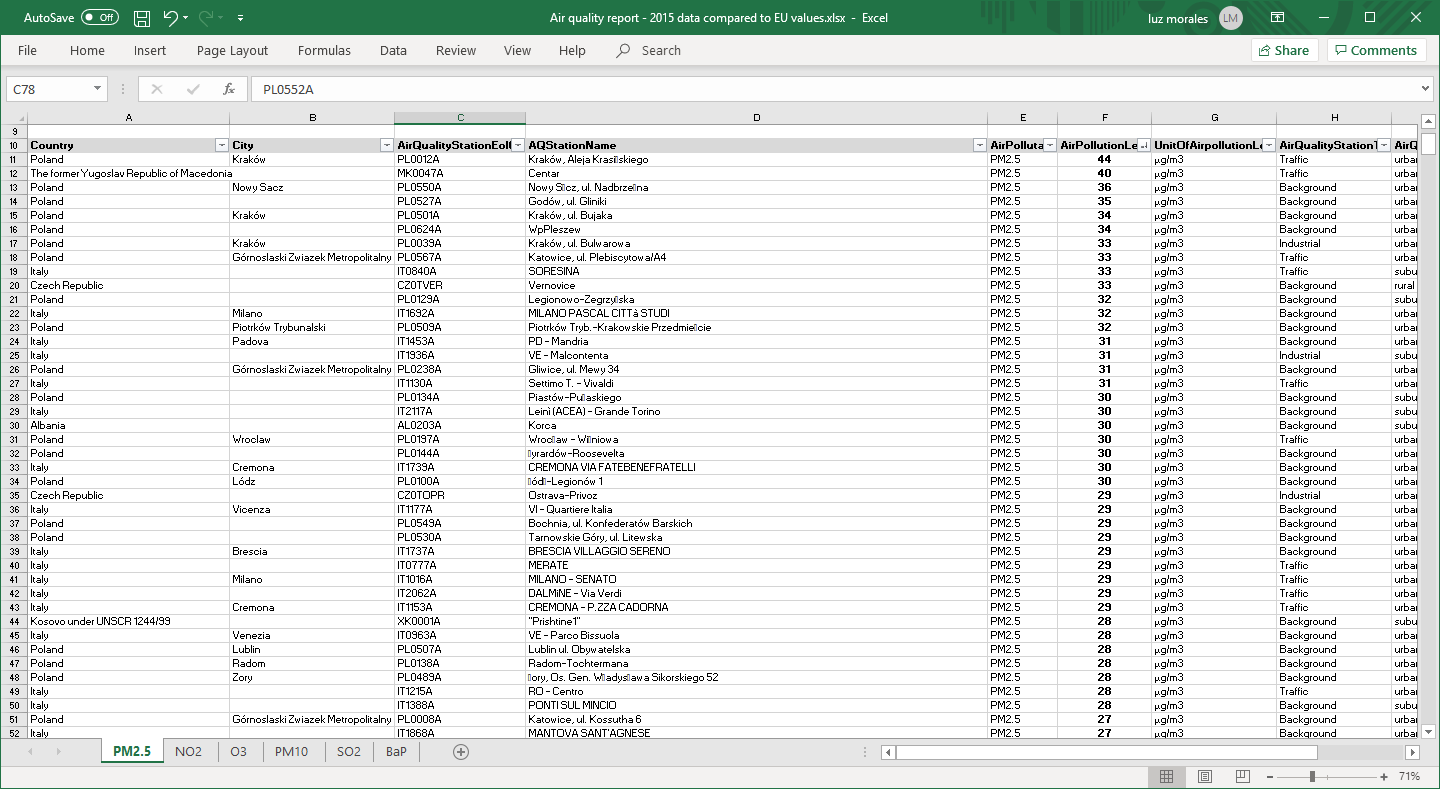
\includegraphics[width=11.5cm]{ExampleOpenDataEuropean}
    \caption{European Open Portal. Air pollutant concentrations 2015} 
   
 
\end{figure}

\newpage
    
A traves de una serie de procesos como son  la extraccion, transformacion y 
limpieza de los datos, se obtendran los datos que se necesitan acorde a nuestro diseno. Estos procesos pueden llegar
a ser muy tediosos si no se automatizan.
Veremos estos procesos en los siguientes apartados\\
    
\noindent\textbf{\textit{Aire Guru} }\\

Los datos extraidos estan en formato GeoJSON, este formato proporciona un objeto JSON con subdocumentos anidados, cada uno de estos
subdocumentos contiene un conjunto de datos en forma clave valor. 
En la siguiente figura podemos ver el principio del documento descargado el 09 de Junio del 2019 
\footnote{\url{https://datosabiertos.malaga.eu/recursos/ambiente/calidadaire/calidadaire.json}}\\
\newpage
\begin{figure}[h]
    \centering
   \subfigure[Primer subdocumento]{ \centering 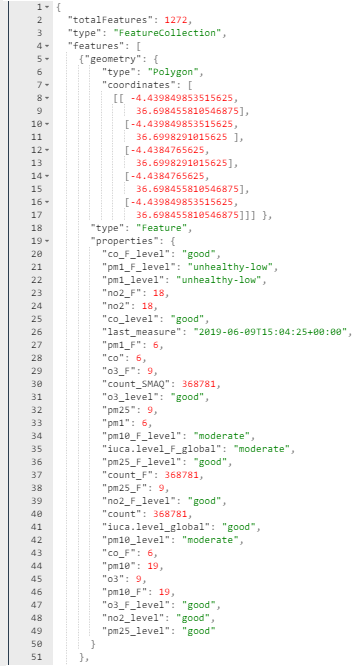
\includegraphics[width=4.75cm]{geoJsonAirQualityData1}}
   \hfill
   \subfigure[Segundo subdocumento]{ \centering 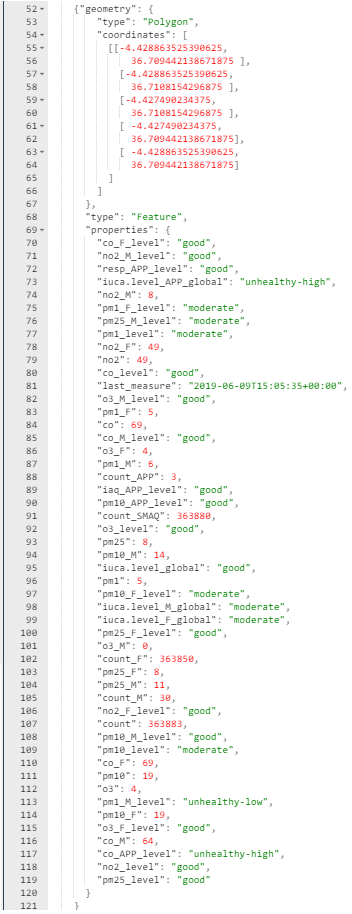
\includegraphics[width=4.75cm]{geoJsonAirQualityData2}}
    \caption{Air quality Document [09/06/2019].Open Data Portal Malaga}
    \end{figure}
    
En este extracto podemos ver los primeros dos subdocumentos. Cada subdocumento contiene las coordenadas de la estacion medidora de la calidad
del aire, la fecha y hora cuando se registro la medida y a continuacion los valores de las mediciones. 
En la figura siguiente podemos encontrar la descripcion proporcionada por el portal de datos abiertos.
\begin{figure}[ht]
    \centering
    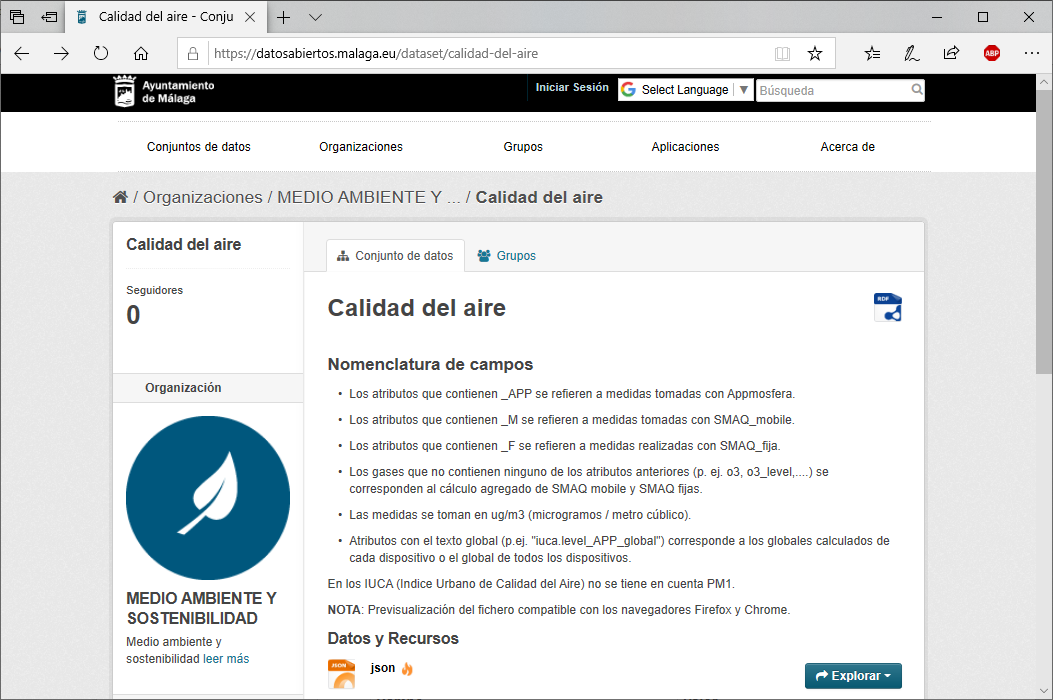
\includegraphics[width=8cm]{geoJsonAirQualityDataDescription}
    \caption{Air quality data description [09/06/2019].Open Data Portal Malaga}
\end{figure}

Para una descripcion mas en detalle de las medidas, tenemos que recurrir a un recurso externo, en este caso nos pusimos en contacto directamente con
la empresa que instala las estaciones de medida UrbanClouds \footnote{\url{https://urbanclouds.city/es/}} y proporciona los datos al ayuntamiento de Malaga.

Una pregunta simple seria saber a que nivel de polucion estamos rodeados en las coordenadas en la que nos encontramos. Con la informacion en 
crudo obtenida desde el portal, nos es una tarea imposible, pero si ardua si no contamos con un sistema que procese los datos.
\begin{itemize}
    \item \textit{Evaluation}
\end{itemize}
